\documentclass[dissertation.tex]{subfiles}
\usepackage[export]{adjustbox}
\usepackage[demo]{graphicx}
\usepackage{caption}
\usepackage{subcaption}

\begin{document}

% \begin{figure}[!htb]
% 	\centering
% 	\begin{subfigure}[t]{0.40\textwidth}
%         \[ \Qcircuit @C=1em @R=.7em {& \targ    & \qw    &\qw  &\cdots & & \qw      & \qw      & \qw &\qw \\
%                                      & \qw      & \targ   &\qw &\cdots & & \qw      & \qw      & \qw &\qw \\
%                         			 & 	     & 	        &          &          & & & & &  &   \\
%                         			 & 	     & 	        &          &          & & & & & \vdots &   \\
%                         			 & \ctrl{-4} & \ctrl{-3}&\qw &\cdots & &\targ   & \qw      & \qw      & \qw \\
%                         			 & \ctrl{-1} & \ctrl{-1}&\qw &\cdots & &\ctrl{-1} & \targ    & \qw      & \qw\\ 
%                         			 & \ctrl{-1} & \ctrl{-1}&\qw &\cdots & &\ctrl{-1} & \ctrl{-1} & \qw      & \qw
% 			  } \]
% 	\caption{Douglas wang increment}
% 	\label{fig:coinedIncrement}
% 	\end{subfigure}

% 	\begin{subfigure}[t]{0.40\textwidth}
%         \[ \Qcircuit @C=1em @R=.7em {& \targ    & \qw      & \qw      & \qw      & \qw \\
%         			  & 	     & 	        &          &          &  . \\
%         			  & 	     & 	        &          &          &  . \\
%         			  & 	     & 	        &          &          &  . \\
%         			  & \ctrlo{-4} & \targ   & \qw      & \qw      & \qw \\
%         			  & \ctrlo{-1} & \ctrlo{-1} & \targ    & \qw      & \qw\\ 
%         			  & \ctrlo{-1} & \ctrlo{-1} & \ctrlo{-1} & \qw      & \qw
% 			  } \]
% 	\centering
% 	\caption{Douglas wang Decrement}
% 	\label{fig:coinedDecrement}
% 	\end{subfigure}
% 	\caption{Douglas wang shift operator}
% 	\label{fig:douglasWangShift}
% \end{figure}

\begin{figure}[]
	\centering
	\begin{adjustbox}{minipage=\linewidth,scale=1}
	\begin{subfigure}[b]{\textwidth}
    \[ \Qcircuit @C=1.5em @R=1.3em { & \qw & \targ    & \qw    &\qw  &\cdots & & \qw      & \qw      & \qw &\qw \\
                                     & \qw & \ctrl{-1}      & \targ   &\qw &\cdots & & \qw      & \qw      & \qw &\qw \\
                        			 & \vdots & 	     & 	        &          &          & & & & &  &   \\
                        			 &  & 	     & 	        &          &          & & & & &  &   \\
                        			 & \qw & \ctrl{-4} & \ctrl{-3}&\qw &\cdots & &\targ   & \qw      & \qw      & \qw \\
                        			 & \qw & \ctrl{-1} & \ctrl{-1}&\qw &\cdots & &\ctrl{-1} & \targ    & \qw      & \qw\\ 
                        			 & \qw & \ctrl{-1} & \ctrl{-1}&\qw &\cdots & &\ctrl{-1} & \ctrl{-1} & \qw      & \qw
			  } \]
	\caption{Douglas wang increment}
	\label{fig:coinedIncrement}
	\end{subfigure}
	
	\begin{subfigure}[b]{\textwidth}
    \[ \Qcircuit @C=1.5em @R=1.3em { & \qw & \targ    & \qw    &\qw  &\cdots & & \qw      & \qw      & \qw &\qw \\
                                     & \qw & \ctrlo{-1}      & \targ   &\qw &\cdots & & \qw      & \qw      & \qw &\qw \\
                        			 & \vdots & 	     & 	        &          &          & & & & &  &   \\
                        			 &  & 	     & 	        &          &          & & & & &  &   \\
                        			 & \qw & \ctrlo{-4} & \ctrlo{-3}&\qw &\cdots & &\targ   & \qw      & \qw      & \qw \\
                        			 & \qw & \ctrlo{-1} & \ctrlo{-1}&\qw &\cdots & &\ctrlo{-1} & \targ    & \qw      & \qw\\ 
                        			 & \qw & \ctrlo{-1} & \ctrlo{-1}&\qw &\cdots & &\ctrlo{-1} & \ctrlo{-1} & \qw      & \qw
			  } \]
	\centering
	\caption{Douglas wang Decrement}
	\label{fig:coinedDecrement}
	\end{subfigure}
	\caption{Douglas wang shift operator}
	\label{fig:douglasWangShift}
	 \end{adjustbox}
\end{figure}

\begin{figure}[!h]
  \centering
  \begin{subfigure}[t]{.4\textwidth}
    \centering
    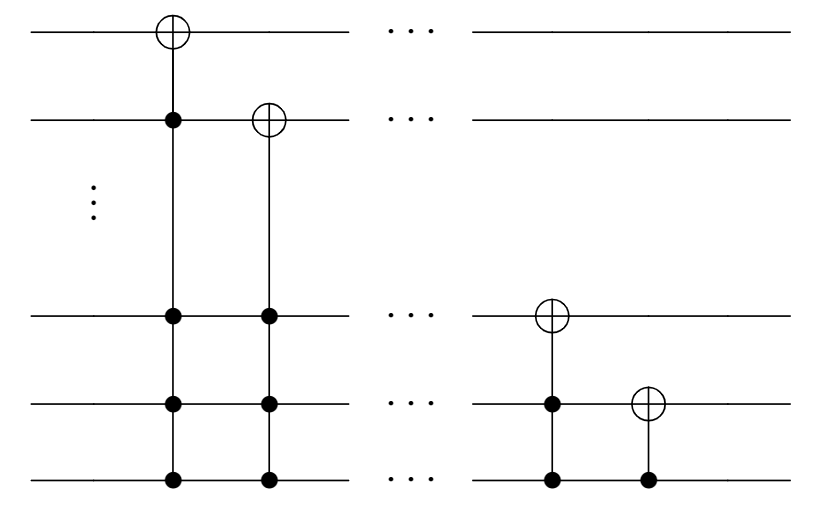
\includegraphics[width=\linewidth]{img/QCircuit/CoinedQuantumWalk/DouglasWangIncrement.png}
    \caption{Increment}
  \end{subfigure}
  %\hfill
  \begin{subfigure}[t]{.4\textwidth}
    \centering
    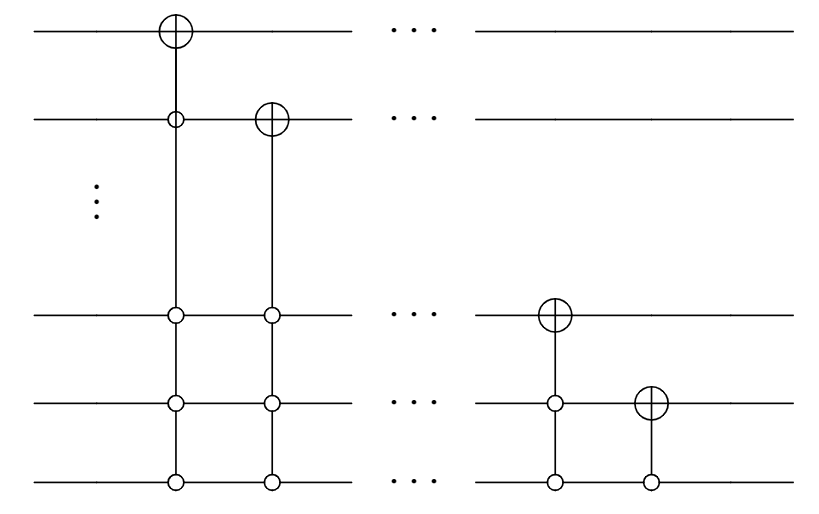
\includegraphics[width=\linewidth]{img/QCircuit/CoinedQuantumWalk/DouglasWangDecrement.png}
    \caption{Decrement}
  \end{subfigure}
  \caption{Shift operators.}
  \label{fig:circulantGraphs}
\end{figure}

\clearpage

\begin{figure}
    \centering
    \[ \Qcircuit @C=1.5em @R=1.3em { & \qw & \targ    & \qw    &\qw  &\cdots & & \qw      & \qw      & \qw &\qw \\
                                     & \qw & \ctrl{-1}      & \targ   &\qw &\cdots & & \qw      & \qw      & \qw &\qw \\
                        			 & \vdots & 	     & 	        &          &          & & & & &  &   \\
                        			 &  & 	     & 	        &          &          & & & & &  &   \\
                        			 & \qw & \ctrl{-4} & \ctrl{-3}&\qw &\cdots & &\targ   & \qw      & \qw      & \qw \\
                        			 & \qw & \ctrl{-1} & \ctrl{-1}&\qw &\cdots & &\ctrl{-1} & \targ    & \qw      & \qw\\ 
                        			 & \qw & \ctrl{-1} & \ctrl{-1}&\qw &\cdots & &\ctrl{-1} & \ctrl{-1} & \qw      & \qw
			  } \]
    \caption{Caption}
    \label{fig:my_label}
\end{figure}

\begin{figure}
    \centering
    \[ \Qcircuit @C=1.5em @R=1.3em { & \qw & \targ    & \qw    &\qw  &\cdots & & \qw      & \qw      & \qw &\qw \\
                                     & \qw & \ctrlo{-1}      & \targ   &\qw &\cdots & & \qw      & \qw      & \qw &\qw \\
                        			 & \vdots & 	     & 	        &          &          & & & & &  &   \\
                        			 &  & 	     & 	        &          &          & & & & &  &   \\
                        			 & \qw & \ctrlo{-4} & \ctrlo{-3}&\qw &\cdots & &\targ   & \qw      & \qw      & \qw \\
                        			 & \qw & \ctrlo{-1} & \ctrlo{-1}&\qw &\cdots & &\ctrlo{-1} & \targ    & \qw      & \qw\\ 
                        			 & \qw & \ctrlo{-1} & \ctrlo{-1}&\qw &\cdots & &\ctrlo{-1} & \ctrlo{-1} & \qw      & \qw
			  } \]
    \caption{Caption}
    \label{fig:my_label}
\end{figure}

\clearpage

% \begin{figure}[!h]
% 	\[ \Qcircuit @C=1em @R=0.7em {         
% 	               &   &\qw      & \multigate{4}{INCR} &  \multigate{4}{DECR} & \qw &\cdots&         &\qw& \multigate{4}{INCR} &  \multigate{4}{DECR} &\qw \\
% 				   &   &\qw      & \ghost{INCR}        & \ghost{DECR}         & \qw &\cdots&         &\qw& \ghost{INCR}       & \ghost{DECR}         &\qw \\
%             	   &	  &\qw      & \ghost{INCR}        & \ghost{DECR}         & \qw &\cdots&         &\qw& \ghost{INCR}      & \ghost{DECR}         &\qw \\
%             	   &\vdots&         & \ghost{INCR}        & \ghost{DECR}         & \qw &\vdots&         & & \ghost{INCR}       & \ghost{DECR}         &\qw \\
%             	   &	  &\qw      & \ghost{INCR}        & \ghost{DECR}         & \qw &\cdots&         &\qw& \ghost{INCR}       & \ghost{DECR}         &\qw \\ 
% 				   &  &\gate{C} & \ctrlo{-1}           & \ctrl{-1}           & \qw &\cdots&         &\qw& \ctrlo{-1}          & \ctrl{-1}           &\qw                  
% 		          } \]
% 	\centering
% 	\caption{Douglas wang coined quantum walk circuit}
% 	\label{fig:coinedCircuit}
% \end{figure}

\begin{figure}[!h]
	\[ \Qcircuit @C=1.5em @R=1.3em {  &&& \mbox{Repeat for the number of steps.} & \\ 
	               &   {/^{\otimes n}}\qw      & \gate{Incr} &  \gate{Decr}    & \qw \\
				   &   \gate{C}                & \ctrlo{-1}           & \ctrl{-1}             & \qw \gategroup{2}{3}{3}{4}{.8em}{--}      
		          } \]
	\centering
	\caption{Douglas wang coined quantum walk circuit}
	\label{fig:coinedCircuit}
\end{figure}

\clearpage

\begin{figure}[!h]
	\[ \Qcircuit @C=1em @R=1em { & \ctrl{2} & \qw & \\
			&\ctrl{1} &\qw & = &  \\
			&\targ & \qw &
		}
		 \Qcircuit @C=1em @R=1em { &\ctrl{2} & \qw  & \qw  & \ctrl{2} & \qw & \ctrl{2} & \qw & \qw\\
				     &\ctrl{1} & \ctrl{1} & \ctrl{1} & \qw & \ctrl{1} & \qw & \ctrl{1} & \qw\\ 
				     &\gate{\phi(\frac{\pi}{2})} & \gate{R_z(\frac{\pi}{2})}  & \gate{R_y(\frac{\pi}{2})} & \targ & \gate{R_y(-\frac{\pi}{2})} & \targ &\gate{R_z(-\frac{\pi}{2})} & \qw 
		          } \]
	\centering
	\caption{Toffoli decomposition}
	\label{fig:toffoliDecompCircuit}
\end{figure}
\pagebreak


\begin{figure}[!h]
	\[ \Qcircuit @C=1.5em @R=1.3em { & \ctrl{5} & \qw & \\
			&\ctrl{4} &\qw & = &  \\
			&         &   &   &  \\
			&         & \vdots  &   &  \\
			&         &   &   &  \\
			&\ctrl{1} &\qw & = &  \\
			&\gate{U} & \qw &  &
		}
			\Qcircuit @C=1.5em @R=1.3em { 
				     &\ctrl{5} & \qw  & \ctrl{6} & \qw & \ctrl{6} & \qw &  \qw\\
				     &\ctrl{4} & \qw & \ctrl{5} & \qw & \ctrl{5} & \qw &  \qw\\ 			
				     &         &         &   &   &  &  \\
				     &         &\vdots         &   & \vdots  &  & \vdots \\
				     &         &         &   &   &  &  \\
				     &\ctrl{1} & \ctrl{1}  & \qw & \ctrl{1} & \qw &\ctrl{1} & \qw \\				     &\gate{\phi} & \gate{A}  & \targ & \gate{B} & \targ &\gate{C} & \qw 
		          } \]
	\centering
	\caption{General decomposition}
	\label{fig:generalDecompCircuit}
\end{figure}
\pagebreak


\begin{figure}[!h]
	\[ \Qcircuit @C=1.5em @R=1.3em { & \ctrl{2} & \qw & \\
			&\ctrl{1} &\qw & = &  \\
			&\targ & \qw &
		}
		 \Qcircuit @C=1em @R=1em { &\ctrl{2} & \qw  & \qw  & \ctrl{2} & \qw & \ctrl{2} & \qw & \qw\\
				     &\ctrl{1} & \ctrl{1} & \ctrl{1} & \qw & \ctrl{1} & \qw & \ctrl{1} & \qw\\ 
				     &\gate{\phi(\frac{\pi}{2})} & \gate{R_z(\frac{\pi}{2})}  & \gate{R_y(\frac{\pi}{2})} & \targ & \gate{R_y(-\frac{\pi}{2})} & \targ &\gate{R_z(-\frac{\pi}{2})} & \qw 
		          } \]
	\centering
	\caption{Toffoli decomposition}
	\label{fig:toffoliDecompCircuit}
\end{figure}

\begin{figure}[!h]
	\[ \Qcircuit @C=1.5em @R=1.3em {& & & & & \mbox{Repeat n times} & &\\
	&\lstick{\ket{qv^{\otimes N}}} & {/} \qw &\gate{H^{\otimes N}}  & \gate{e^{i\gamma\frac{Ot}{n}^{\otimes N}}} & \gate{F^{\otimes N}} &\gate{e^{i\gamma\frac{\Lambda t}{n}^{\otimes N}}} & \gate{F^{\dagger^{\otimes N}}} &\qw \gategroup{2}{5}{2}{8}{.8em}{--}
		          } \]
	\centering
	\caption{Temp}
	\label{fig:contSearchCircuit}
\end{figure}\

\begin{figure}[!h]
	\[ \Qcircuit @C=1.8em @R=1.5em {& & & &\mbox{t times}  & & && &\\
	&\lstick{\ket{0^{\otimes n}}} & {/} \qw &\gate{H^{\otimes n}}  & \gate{O_M} &  \gate{G} &{/}\qw &\qw \gategroup{2}{5}{2}{6}{.8em}{--}
		          } \]
	\centering
	\caption{Temp}
	\label{fig:contSearchCircuit}
\end{figure}
\pagebreak

\begin{figure}[!h]
	\[ \Qcircuit @C=1em @R=0.7em { 
	               &       &\qw & \qw      & \multigate{4}{INCR}&\qw &  \multigate{4}{DECR} & \qw &\cdots&         &\qw& \qw& \multigate{4}{INCR}&\qw &  \multigate{4}{DECR} &\qw \\
				   &       &\qw & \qw   & \ghost{INCR}      &\qw     & \ghost{DECR}         & \qw &\cdots&         &\qw&\qw& \ghost{INCR}&\qw       & \ghost{DECR}         &\qw \\
            	   &	   &\qw & \qw    & \ghost{INCR}      &\qw    & \ghost{DECR}         & \qw &\cdots&         &\qw&\qw& \ghost{INCR}&\qw      & \ghost{DECR}         &\qw \\
            	   &\vdots &    &      & \ghost{INCR}       &\qw     & \ghost{DECR}         & \qw &\vdots&         & \qw&\qw & \ghost{INCR} &\qw      & \ghost{DECR}         &\qw \\
            	   &  &\qw & \gate{R_x(2\theta)}    & \ghost{INCR} &\gate{R_x(2\theta)}        & \ghost{DECR}         & \qw &\cdots&         &\qw&\gate{R_x(2\theta)}& \ghost{INCR}&\gate{R_x(2\theta)}       & \ghost{DECR}         &\qw \\ 
		          } \]A
	\caption{stagqw}
	\label{fig:stagqw}
\end{figure}

\begin{figure}[!h]
	\[ \Qcircuit @C=1em @R=0.7em {   & & && \mbox{Repeat for the number of steps} & &\\\\
	               &       & \qw & {/^{\otimes n-1}}\qw      & \multigate{1}{INCR}&\qw &  \multigate{1}{DECR} & \qw \\
            	   &       &\qw & \gate{R_x(2\theta)}    & \ghost{INCR} &\gate{R_x(2\theta)}        & \ghost{DECR} & \qw \gategroup{3}{4}{4}{7}{.8em}{--} 
		          } \]A
	\caption{stagqw}
	\label{fig:stagqw}
\end{figure}

\begin{figure}[!h]
	\[ \Qcircuit @C=1.8em @R=1.5em {
	& & {/^{\otimes n}} \qw &\gate{QFT_m}  & \gate{e^{i\gamma\Lambda t}} &  \gate{QFT^{\dagger}_m} &\qw &\qw 
		          } \]
	\centering
	\caption{Temp}
	\label{fig:contCircuit}
\end{figure}

\begin{figure}[!h]
	\[ \Qcircuit @C=1.8em @R=1.5em { &&&& \mbox{Repeat $O(\sqrt{N})$ times.} & &\\
	&\lstick{\ket{\psi_0}} & {/^{\otimes n}} \qw&\gate{O} &\gate{H}  & \gate{e^{i\theta\mathcal{O}_0}} &  \gate{H} &\qw &\qw \gategroup{2}{4}{2}{7}{.8em}{--} \\
		          } \]
	\centering
	\caption{Temp}
	\label{fig:stagSearchCircuit}
\end{figure}

% \begin{figure}[!h]
% 	\[ \Qcircuit @C=1.8em @R=1.5em {& & & & \mbox{ O(\sqrt{N}) times}  & & &\\
% 	& & {/^{\otimes n}} \qw &\gate{H}  & \gate{O_M} &  \gate{G} & \qw &\qw \gategroup{2}{5}{2}{6}{.8em}{--}
% 		          } \]
% 	\centering
% 	\caption{Temp}
% 	\label{fig:groverSearchCircuit}
% \end{figure}

\begin{figure}[!h]
	\[ \Qcircuit @C=1.8em @R=1.5em { & & & & \mbox{ Repeat $O(\sqrt{N})$ times}  &\\
	                                & {/^{\otimes n}} \qw  &\gate{H}  & \gate{\mathcal{O}} & \multigate{1}{SHIFT} & \qw &  \\
				                    & {/^{\otimes n}} \qw  & \qw & \gate{G}&   \ghost{SHIFT} & \qw \gategroup{2}{4}{3}{5}{.8em}{--}
		          } \]
	\centering
	\caption{Douglas wang coined quantum walk circuit}
	\label{fig:coinedSearchCircuit}
\end{figure}
\clearpage

\begin{figure}[!h]
	\[ \Qcircuit @C=1.5em @R=1.3em { 
	               &   & \multigate{1}{\Delta} &\qw  & &\raisebox{-2.2em}{\equiv} & \\
				   &  {/} &\ghost{\Delta} &\qw
		          } 
		\Qcircuit @C=1.5em @R=1.0em { 
	               &        &\qw     & \gate{Rz} \cwx[1] & \qw \\
				   & {/} & \gate{\Delta}    & \controlo  \qw   & \qw     
		          }\]
	\centering
	\caption{Decomposition of diagonal operators.}
	\label{fig:coinedCircuit}
\end{figure}

\clearpage

\begin{figure}[!h]
	\[ \Qcircuit @C=1.5em @R=1.3em { 
	               & \gate{R_z} \cwx[1] &\qw   &\raisebox{-2.2em}{\equiv} & \\
				   & \controlo  \qw  &\qw
		          } 
		\Qcircuit @C=1.5em @R=1.3em { 
	               & \gate{R_z} &\targ         & \gate{R_z} & \targ    & \qw \\
				   & \qw        & \ctrl{-1}    &  \qw       & \ctrl{-1} & \qw    
		          }\]
	\centering
	\caption{Decomposition of a singly-multiplexed $R_z$ gate.}
	\label{fig:coinedCircuit}
\end{figure}

\clearpage

\begin{figure}[!h]
	\[ \Qcircuit @C=1.5em @R=1.3em { 
	              & & \gate{R_z} \cwx[1]        &\qw   &&\raisebox{-4.5em}{\equiv} & \\
				  &{/} & \controlo \cwx[1] \qw  &\qw\\
				  &   & \controlo  \qw          &\qw
		          } 
		\Qcircuit @C=1.5em @R=1.3em { 
	               &   & \gate{R_z} \cwx[1] &\targ         & \gate{R_z}\cwx[1] & \targ    & \qw \\
				   &{/}& \controlo \qw      & \qw          &  \controlo \qw    & \qw & \qw\\
                   &   & \qw                & \ctrl{-2}    &  \qw             & \ctrl{-2} & \qw    
		          }\]
	\centering
	\caption{General decomposition of a multiplexed $R_z$ gate.}
	\label{fig:coinedCircuit}
\end{figure}


\end{document}
